%\newcommand{\ein}[2]{(#1) (#2 Punkte)}


\begin{Large}
\textbf{Teil I: Offene Fragen (38 Punkte)}
\end{Large}
\\
\\
\\
\textbf{Allgemeine Anweisungen für offene Fragen:}
\\
\renewcommand{\labelenumi}{(\roman{enumi})}
\begin{enumerate}
\item
Ihre Antworten müssen alle Rechenschritte enthalten,
diese müssen klar ersichtlich sein.
Verwendung korrekter mathematischer Notation wird erwartet
und fliesst in die Bewertung ein.

\item
Ihre Antworten zu den jeweiligen Teilaufgaben müssen in den dafür vorgesehenen Platz geschrie-
ben werden. Sollte dieser Platz nicht ausreichen, setzen Sie Ihre Antwort auf der Rückseite oder
dem separat zur Verfügung gestellten Papier fort. Verweisen Sie in solchen Fällen ausdrücklich
auf Ihre Fortsetzung. Bitte schreiben Sie zudem Ihren Vor- und Nachnamen auf jeden separaten
Lösungsbogen.

\item
Es werden nur Antworten im dafür vorgesehenen Platz bewertet. Antworten auf der Rückseite
oder separatem Papier werden nur bei einem vorhandenen und klaren Verweis darauf bewertet.

\item
Die Teilaufgaben werden mit den jeweils oben auf der Seite angegebenen Punkten bewertet.

\item
Ihre endgültige Lösung jeder Teilaufgabe darf nur eine einzige Version enthalten.

\item
Zwischenrechnungen und Notizen müssen auf einem getrennten Blatt gemacht werden. Diese
Blätter müssen, deutlich als Entwurf gekennzeichnet, ebenfalls abgegeben werden.
\end{enumerate}

\newpage
\section*{\hfil Aufgaben \hfil}
\vspace{1cm}
\section*{Aufgabe 1 (38 Punkte)}
\vspace{0.4cm}
%\titleformat{\subsection}[runin]
%{\normalfont\large\bfseries}{\thesubsection}{1em}{}
\subsection*{\aufgabe{a1}{8}} 
Die durchschnittlichen jährlichen Stromkosten eines Schweizer Haushalts sind von ungefähr $800$ Schweizer Franken im Jahr $2012$ auf (voraussichtlich) $1'200$ Schweizer Franken im Jahr $2023$ gestiegen. Um diese Entwicklung darzustellen, nehmen wir an, dass sich die Kosten $C$ über die Zeit gemäss dem folgenden mathematischen Modell entwickeln:
\begin{align*}
	C_\lambda(t)
	=
	\frac{1600}{1 + e^{-\lambda t}},
\end{align*}
wobei $t \geq 0$ die Anzahl der Jahre \textit{nach} $2012$ entspricht und $\lambda = 0.1$.
\\
\\
Nehmen wir an, dass man die Preisentwicklung durch eine Verbesserung der Energieeffizienz entgegenwirken kann, was durch den Parameter $\lambda$ ausgedrückt wird. Das heisst, die Kosten im Jahr $2023$ können beschrieben werden als:
\begin{align*}
	c_{2023}(\lambda) 
	=
	\frac{1600}{1 + e^{- \lambda (2023 - 2012)}}.
\end{align*}
Zeigen Sie, dass es genau einen Wert $\lambda^\star \in [0,0.1]$ gibt, bei dem die Kosten im Jahr $2023$ $1'000$ Schweizer Franken entsprechen.

\subsection*{\aufgabe{a2}{8}}
Die durchschnittlichen jährlichen Stromkosten eines Schweizer Haushalts sind von ungefähr $800$ Schweizer Franken im Jahr $2012$ auf (voraussichtlich) $1'200$ Schweizer Franken im Jahr $2023$ gestiegen. Um diese Entwicklung darzustellen, nehmen wir an, dass sich die Kosten $C$ über die Zeit gemäss dem folgenden mathematischen Modell entwickeln:
\begin{align*}
	C_\lambda(t)
	=
	\frac{1600}{1 + e^{-\lambda t}},
\end{align*}
wobei $t \geq 0$ die Anzahl der Jahre \textit{nach} $2012$ entspricht und $\lambda = 0.1$.
\\
\\
Nehmen wir an, dass man die Preisentwicklung durch eine Verbesserung der Energieeffizienz entgegenwirken kann, was durch den Parameter $\lambda$ ausgedrückt wird. Das heisst, die Kosten im Jahr $2023$ können beschrieben werden als:
\begin{align*}
	c_{2023}(\lambda) 
	=
	\frac{1600}{1 + e^{- \lambda (2023 - 2012)}}.
\end{align*}
Verwenden Sie eine Taylor-Approximation zweiter Ordnung im Punkt $ \lambda_0 = 0.05 $, um eine Näherung für $ \lambda^\star $ zu finden.
 \\
\\
\titleformat{\subsection}[display]
{\normalfont\large\bfseries}{\thesubsection}{1mm}{}
\subsection*{\aufgabe{b}{12}}
Sam begeistert sich für non-fungible tokens (NFTs).
Er beschliesst ein digitales Kunstwerk zu kaufen, da er fest daran glaubt, dass der Wert des Kunstwerks innerhalb der nächsten Jahre signifikant steigen wird. 
Das NFT Kunstwerk kostet $100'000$ Schweizer Franken und Sam
beschliesst, sich einen Teil des Geldes für die Finanzierung zu leihen.
Eine Freundin, Caroline, willigt ein, ihm zum 1. Januar 2023 $60'000$
Schweizer Franken zu leihen, wodurch $60 \% $ der Kosten gedeckt werden.
Allerdings verlangt sie einen recht hohen jährlichen Zinssatz
von $5 \%$, da sie Sams Investitionsvorhaben eher skeptisch gegenübersteht.
Darüber hinaus besteht sie darauf, dass Sams Schulden bis Ende des Jahres 2025 auf
$30'000$ Schweizer Franken gesunken und schliesslich bis Ende des Jahres 2028 vollständig getilgt sind.
Um diese Bedingungen zu erfüllen, stimmt Sam zu, dass er jedes Jahr, jeweils am Jahresende, bis zum 31. Dezember 2025 $C_1$ zurückzahlt und $C_2 = 5'000$ Schweizer Franken am Ende jeden Jahres vom 1. Januar 2026 bis zum 31. Dezember 2028.
Die verbleibenden Schulden am Ende des Jahres 2028 will er dann mit dem durch den Verkauf des Kunstwerks generierten
Erlös zurückzahlen.
\begin{enumerate}
	\item[(b1)] Fügen Sie die Ereignisse und Mittelflüsse dem Zeitstrahl hinzu.
	\item[(b2)] Bestimmen Sie die jährlichen Zahlungen $C_1$ jeweils am Ende der Jahre 2023, 2024 und 2025.
	\item[(b3)] Bestimmen Sie die Restschuld am Ende des Jahres 2028 \textit{bevor} Sam das Kunstwerk verkaufen und die Schulden vollständig tilgen wird.
	\item[(b4)] Angenommen Sams Erwartungen bezüglich der Wertentwicklung seines NFT Kunstwerks waren falsch und das Kunstwerk hat seit 1. Januar 2023 jährlich $3 \%$ an Wert verloren. Prüfen Sie, ob es Sam möglich ist, seine Schulden vollständig zurückzuzahlen, wenn er \textit{ausschliesslich} seine Einnahmen aus dem Verkauf des Kunstwerks dafür verwendet.
\end{enumerate}
\begin{center}
	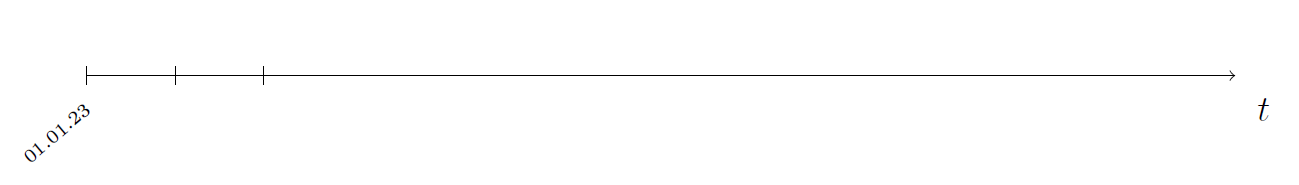
\includegraphics[scale=0.45]{pictures/zeitstrahl_1_b}
\end{center}
\newpage
\subsection*{\aufgabe{c}{10}}
Die Alterung der Bevölkerung hat bedeutende ökonomische und soziale Auswirkungen. Deshalb ist es für die Politik von hoher Bedeutung, ein umfassendes Verständnis davon zu haben, wie sich das Bevölkerungswachstum über die nächsten 50 Jahre entwickeln wird.
Modelle des Bevölkerungswachstums sind eine mathematische Beschreibung, wie die Bevölkerung voraussichtlich in Zukunft wachsen wird.
Eines dieser Modelle nimmt an, dass sich die Grösse $s(t)$ einer Bevölkerung zum Zeitpunkt $t \geq 0$ durch die folgende mathematische Formel beschreiben lässt:
\begin{align*}
	s(t)
	=
	\left(s_0^{1- \gamma} + \mu (1 - \gamma)  t \right)^{\frac{1}{1- \gamma}},
\end{align*}
wobei $s_0 = s(0)$ die Grösse der Bevölkerung zum Zeitpunkt $0$ ist und $\mu, \gamma > 0, \ \gamma \neq 1$ gegebene Parameter sind.
\begin{enumerate}
	\item[(c1)] Berechnen Sie die Wachstumsrate $ \rho_s(t) $ von $ s $.
	\item[(c2)] Benutzen Sie unter der Annahme, dass $s(0) = 10'000 $ Individuen, $\mu = 10$, und $\gamma = 0.5$, die Ableitung von $s$, um die relative Änderung der Bevölkerung zwischen dem Zeitpunkt $t_0 = 5 $ und dem Zeitpunkt $t_0 + \Delta t = 6$ zu approximieren.
\end{enumerate}


\newpage


\fancyhead[C]{\normalsize\textbf{$\qquad$ Teil II: Multiple-Choice}}
\begin{Large}
\textbf{Teil II: Multiple-Choice-Fragen (62 Punkte)}
\end{Large}
\\
\\
\\
\textbf{Allgemeine Anweisungen für Multiple-Choice-Fragen:}
\\
\renewcommand{\labelenumi}{(\roman{enumi})}
\begin{enumerate}
\item
Die Antworten auf die Multiple-Choice-Fragen müssen im dafür vorgesehenen Antwortbogen ein-
getragen werden. Es werden ausschliesslich Antworten auf diesem Antwortbogen bewertet. Der
Platz unter den Fragen ist nur für Notizen vorgesehen und wird nicht korrigiert.

\item
Jede Frage hat nur eine richtige Antwort. Es muss also auch jeweils nur eine Antwort angekreuzt werden.

\item
Falls mehrere Antworten angekreuzt sind, wird die Antwort mit 0 Punkten bewertet, auch wenn
die korrekte Antwort unter den angekreuzten ist.

\item
Bitte lesen Sie die Fragen und die Anweisungen auf dem Multiple-Choice-Antwortbogen sorgfältig.

\end{enumerate}

\section*{Aufgabe 2 (34 Punkte)}
\vspace{0.4cm}

\subsection*{\frage{1}{3}}
$ A $ und $ B $ seien zwei Aussagen. Welche der folgenden zwei zusammengesetzten Aussagen sind äquivalent? 
 \renewcommand{\labelenumi}{(\alph{enumi})}
\begin{enumerate}
\item $ A \Rightarrow  B $ und $A \vee B$.
\item $ A \vee B $ und $\neg (A \vee B)$.
\item $ (A \Rightarrow \neg B) $ und $\neg ( A \vee B )$
\item Keine der obigen Antworten ist richtig.
\end{enumerate}
\ \\
\subsection*{\frage{2}{4}}
Welche der folgenden zusammengesetzten Aussagen ist eine Tautologie? 
\renewcommand{\labelenumi}{(\alph{enumi})}
\begin{enumerate}
	\item $(A \Rightarrow B ) \wedge (B \Rightarrow A)$.
	\item $ ((A \wedge B) \Rightarrow B) \vee A$.
	\item $ ((A \vee B) \Rightarrow B) \vee B$
	\item $(A \Rightarrow B ) \vee \neg A \vee B$.
\end{enumerate}
\ \\
\subsection*{\frage{3}{3}}
Seien $\{a_k\}_{k \in \mathbb{N}}$ und $\{b_k\}_{k \in \mathbb{N}}$ zwei geometrische Folgen mit $a_1 = 1$, $a_2= 1.01$ und $b_1 = 3$, $b_2 = -2$.\\
\\
Welche der folgenden Aussagen ist korrekt? 
\renewcommand{\labelenumi}{(\alph{enumi})}
\begin{enumerate}
\item 
$\{a_k\}_{k \in \mathbb{N}}$ und $\{b_k\}_{k \in \mathbb{N}}$ konvergieren beide.
\item 
Nur $\{a_k\}_{k \in \mathbb{N}}$ konvergiert.
\item 
Nur $\{b_k\}_{k \in \mathbb{N}}$ konvergiert.
\item
Weder $\{a_k\}_{k \in \mathbb{N}}$ noch $\{b_k\}_{k \in \mathbb{N}}$ konvergieren.
\end{enumerate}
\ \\
\subsection*{\frage{4}{4}}
Seien $\{a_k\}_{k \in \mathbb{N}}$ und $\{b_k\}_{k \in \mathbb{N}}$ zwei geometrische Folgen mit $a_1 = 1$, $a_2= 1.1$ und $b_1 = 3$, $b_2 = 3.1$.
Seien $\{s_n^a \}_{n \in \mathbb{N}}$ und $\{s_n^b \}_{n \in \mathbb{N}}$ die entsprechenden Reihen.\\
\\
Welche der folgenden Aussagen ist korrekt? 
\renewcommand{\labelenumi}{(\alph{enumi})}
\begin{enumerate}
	\item 
	$\lim_{n \to \infty} \frac{s_n^a}{s_n^b} = 3$.
	\item
	$\lim_{n \to \infty} \frac{s_n^a}{s_n^b} = \frac{1}{3}$.
	\item
	$\lim_{n \to \infty} \frac{s_n^a}{s_n^b} = \infty$.
	\item
	$\lim_{n \to \infty} \frac{s_n^a}{s_n^b} = 0$.
\end{enumerate}
\ \\
\subsection*{\frage{5}{3}}
Ein Projekt erfordert eine Anfangsinvestition von $10'000$ Schweizer Franken und generiert Erträge in Höhe von $500$ Schweizer Franken am Ende jedes Jahres für $10$ Jahre, sowie zusätzliche $12'000$ Schweizer Franken am Ende des zehnten Jahres.\\
\\
Der interne Zinssatz des Projekts ist:
\renewcommand{\labelenumi}{(\alph{enumi})}
\begin{enumerate}
	\item 
	Echt grösser als $5 \%$.
	\item 
	Gleich $5 \%$.
	\item
	Echt kleiner als $5 \%$.
	\item
	Die Frage kann nicht beantwortet werden, ohne zu wissen, welcher Zinssatz $i$ gilt.
\end{enumerate}
\ \\
\subsection*{\frage{6}{3}}
Seien $h$, $f$ und $g$ differenzierbare Funktionen einer reellen Variable. Welche der folgenden Formeln ist korrekt?
\renewcommand{\labelenumi}{(\alph{enumi})}
\begin{enumerate}
	\item 
	$ \frac{d}{dx}h(f(x) + g(x)) = h^\prime(x) ( f^\prime(x) + g^\prime(x))$.
	\item 
	$ \frac{d}{dx}h(f(x) + g(x)) = h^\prime(x) ( f(x) + g(x))^\prime$.
	\item
	$ \frac{d}{dx}h(f(x) + g(x)) = h^\prime(f(x))  f^\prime(x) + h^\prime(g(x)) g^\prime(x)$.
	\item
	$ \frac{d}{dx}h(f(x) + g(x)) = h^\prime(f(x) + g(x))  (f^\prime(x) +  g^\prime(x) )$.
	\item
	$ \frac{d}{dx}h(f(x) + g(x)) = h^\prime(f(x) + g(x))  f^\prime(x)  g^\prime(x)$.
\end{enumerate}
\ \\
\subsection*{\frage{7}{4}}
Welche der folgenden Aussagen ist korrekt für eine differenzierbare Funktion $f$ auf einem Intervall $[a,b]$ und $x_0 \in (a,b)$?
\renewcommand{\labelenumi}{(\alph{enumi})}
\begin{enumerate}
\item 
$x_0$ ist genau dann ein stationärer Punkt, wenn er ein Extrempunkt ist.
\item
Wenn $x_0$ ein Wendepunkt ist, dann ist er auch ein stationärer Punkt.
\item
Wenn $x_0$ der einzige lokale Extrempunkt in $(a,b)$ ist, dann ist er auch ein globaler Extrempunkt in $[a,b]$.
\item
Wenn $f^\prime(x_0) = 0$, dann ist $x_0$ ein Extrempunkt.
\item
Keine der obigen Antworten ist richtig.
\end{enumerate}
\ \\
\subsection*{\frage{8}{3}}
Seien $f$ und $g$ konkave, zweimal differenzierbare Funktionen. Welche der folgenden Aussagen ist korrekt?
\renewcommand{\labelenumi}{(\alph{enumi})}
\begin{enumerate}
	\item 
	$f \ g$ ist konkav.
 	\item
	$f \ g$ ist konvex.
	\item
	$f \circ g $ ist konkav.
	\item
	$f +g $ ist konvex.
	\item 
	$f+g$ ist konkav.
\end{enumerate}
\ \\
\subsection*{\frage{9}{3}}
Sei $f$ eine differenzierbare Funktion. Welcher der folgenden Ausdrücke approximiert 
$x_0 \frac{f(x_0 + \Delta x) - f(x_0)}{f(x_0) \Delta x}$, wenn $\Delta x$ klein ist?
\renewcommand{\labelenumi}{(\alph{enumi})}
\begin{enumerate}
	\item 
	Die Ableitung $f^\prime(x_0)$.
	\item
	Die Änderungsrate $\rho_f(x_0)$.	
	\item
    Das Differential $df$.
	\item
	Die Elastizität $\varepsilon_f(x_0)$.
\end{enumerate}
\ \\
\subsection*{\frage{10}{4}}
Sei $f$ eine Funktion und $x_0 \in D_f$ so, dass $f(x_0) = 1$ und $f^{(k)}(x_0) = 1$ für $k = 1,2,3$ gilt. Seien $P_2$ und $P_3$ jeweils das Taylor-Polynom zweiter und dritter Ordnung von $f$ in $x_0$. Es folgt, dass:
\renewcommand{\labelenumi}{(\alph{enumi})}
\begin{enumerate}
	\item 
	$P_3(x) - P_2(x) = 0 $ für alle $x$.
	\item
	$P_3(x) - P_2(x) = (x - x_0)^2 $ für alle $x$.
	\item
	$P_3(x) - P_2(x) = \frac{1}{6} (x - x_0)^3 $ für alle $x$.
	\item
	Es ist nicht möglich die Frage zu beantworten, ohne die Funktionsvorschrift von $f$ zu kennen.
\end{enumerate}


\newpage
\section*{Aufgabe 3 (28 Punkte)}
\vspace{0.4cm}

\subsection*{\frage{1}{3}}
Welche der folgenden Folgen konvergiert gegen $1$?
\renewcommand{\labelenumi}{(\alph{enumi})}
\begin{enumerate}
	\item 
	$ \{a_n\}_{n \in \mathbb{N}} $ mit $a_n = \frac{\sin(n) - \cos(n)}{n}$.
	\item
	$ \{b_n\}_{n \in \mathbb{N}} $ mit $b_n = \frac{n^2}{2n^2 - 3n +1 }$.
	\item
	$ \{c_n\}_{n \in \mathbb{N}} $ mit $c_n = \sqrt{n^2 + 1 }  - n$.
	\item
	$ \{d_n\}_{n \in \mathbb{N}} $ mit $d_n = \frac{n^2}{e^n}$.
	\item
	$ \{e_n\}_{n \in \mathbb{N}} $ mit $e_n = \frac{(n+2)(n^2 + 3n -1 )}{n^3 + 4 }$.
	\item
	$ \{f_n\}_{n \in \mathbb{N}} $ mit $f_n = \frac{\ln(n)}{n}$.
\end{enumerate}
\ \\
\subsection*{\frage{2}{4}}
Welche der folgenden Konditionen ist am besten?
\renewcommand{\labelenumi}{(\alph{enumi})}
\begin{enumerate}
	\item 
	Jährlicher Zinssatz von $5 \%$ mit jährlicher Verzinsung.
	\item
	Jährlicher Zinssatz von $4.95 \%$ mit halbjährlicher Verzinsung.
	\item
	Jährlicher Zinssatz von $4.9 \%$ mit vierteljährlicher Verzinsung.
	\item
	Jährlicher Zinssatz von $4.85 \%$ mit monatlicher Verzinsung.
	\item
	Jährlicher Zinssatz von $4.8 \%$ mit stetiger Verzinsung.	
\end{enumerate}
\ \\
\subsection*{\frage{3}{4}}
Gegeben ist die Funktion
\begin{align*}
	f(x) = \sin(\ln(x^2 + x + 1)).
\end{align*}
Die Ableitung von $f$ in $x_0 = 0 $ ist:
\renewcommand{\labelenumi}{(\alph{enumi})}
\begin{enumerate}
	\item 
	$ 0$.
	\item
	$ 1 $.
	\item
	$ 2 $.
	\item
	$ \pi $.
	\item
	$f$ ist nicht differenzierbar in $x_0 = 0$.
\end{enumerate}
\ \\
\subsection*{\frage{4}{4}}
Sei $P_3$ das Taylor-Polynom dritter Ordnung von $f(x) = \ln(1+ x) $ in $x_0 = 0$.\\
\\
Es gilt, dass:
\renewcommand{\labelenumi}{(\alph{enumi})}
\begin{enumerate}
\item 
$P_3(1) = 1 $.
\item 
$P_3(1) = \frac{1 }{2}$.
\item
$P_3(1) =  0$.
\item
$P_3(1) = \frac{1 }{6}$.
\item
$P_3(1) = \frac{5 }{6}$.
\end{enumerate}
\ 
\subsection*{\frage{5}{3}}
Sei $f$ die Funktion zweier reeller Variablen definiert durch $f(x,y) = \cos(x^2 +y^2 + 2xy).$\\
\\
Die partiellen Ableitungen von $f$ in $(x_0, y_0) = \left(\sqrt{\frac{\pi}{2}}, \sqrt{\frac{\pi}{2}}\right)$ sind:
\renewcommand{\labelenumi}{(\alph{enumi})}
\begin{enumerate}
\item 
$f_x(x_0,y_0) = 0$ und $f_y(x_0,y_0) = 0$.
\item
$f_x(x_0,y_0) = 4 \sqrt{\frac{\pi}{2}} $ und $f_y(x_0,y_0) = 0$.
\item
$f_x(x_0,y_0) = 0 $ und $f_y(x_0,y_0) = 4 \sqrt{\frac{\pi}{2}}$.
\item
$f_x(x_0,y_0) = 4 \sqrt{\frac{\pi}{2}} $ und $f_y(x_0,y_0) = 4 \sqrt{\frac{\pi}{2}}$.
\end{enumerate}
\ \\
\subsection*{\frage{6}{4}}
Wir betrachten die Gleichung
\begin{align*}
	\ln(x) + x y^2 + \frac{2x}{x + 2y} - 2 = 0,
\end{align*}
die für $(x_0,y_0) = (1,0)$ erfüllt ist.\\
\\
Die marginale Änderung in $y$, wenn $x$ ausgehend von $x_0$ marginal geändert wird und die Gleichung weiterhin erfüllt ist, ist:
\renewcommand{\labelenumi}{(\alph{enumi})}
\begin{enumerate}
	\item 
	$ 0 $.
	\item
	$ \frac{1}{4}$.
	\item
	$ -\frac{1}{4}$.
	\item
	$ 1$.
	\item
	Keine der obigen Antworten ist korrekt.
\end{enumerate}
\ \\
\subsection*{\frage{7}{2}}
Gegeben ist die Funktion
\begin{align*}
	f(x,y) 
	=
	2 x^3 e^{\frac{ 2x^2+y^2}{x^2 - 3y^2 }}
	-
	xy^2 e^{\frac{x+y}{x-y}}
	+
	x y^3 \ln \left( \frac{x+y }{2y} \right)
	\quad \textrm{für } x>0,y>0.
\end{align*}
Welche der folgenden Aussagen ist korrekt?
\renewcommand{\labelenumi}{(\alph{enumi})}
\begin{enumerate}
	\item
	$ f  $ ist homogen vom Grad $ 0 $.
	\item
	$ f  $ ist homogen vom Grad $ 2 $.
	\item
	$ f  $ ist homogen vom Grad $ 2 $..	
	\item 
	$ f  $ ist homogen vom Grad $ 4 $.
	\item
	$ f $ ist nicht homogen.
\end{enumerate}
\ \\
\subsection*{\frage{8}{4}}
Gegeben ist die Funktion
\begin{align*}
	f(x,y)
	=
	\frac{x^{3a} y^b}{x^3 +y^3} e^{\frac{x^a y}{y^{a+1}}}
	- 
	\frac{1}{x^3 y^{3b} + x y^{2 + 3b}},
\end{align*}
wobei $ x > 0, y > 0 $ und $ a,b \in \R $.\\
\\
Für welche Werte von $ a $ und $ b $ gilt
\begin{align*}
	\varepsilon_x(x,y) + \varepsilon_y(x,y) = 2 \ \textrm{für alle } x>0, y>0\textrm{?}
\end{align*}
\renewcommand{\labelenumi}{(\alph{enumi})}
\begin{enumerate}
	\item 
	$a = \frac{10}{9}$ und $ b=-\frac{5}{3} $.
	\item
	$a = \frac{17}{9}$ und $ b=-\frac{2}{3} $.
	\item
	$a = \frac{20}{9}$ und $ b=-\frac{5}{3} $.
	\item
	$a = \frac{20}{9}$ und $ b=-\frac{2}{3} $.
	\item
	$a = \frac{19}{9}$ und $ b=-\frac{5}{3} $.
	\item
	Es gibt keine Kombination $ a $ und $ b $, die die Bedingung erfüllt.
\end{enumerate}